\documentclass[12pt]{article}
\usepackage{setspace, graphicx, fullpage, amssymb, amsmath, epsfig, natbib, array, multirow, hyperref}
\usepackage{amsfonts, bm} 
\usepackage{dcolumn}
\usepackage{subfigure, float} 
\usepackage[margin=1.25in]{geometry} 
\usepackage{verbatim}
\usepackage{url}
\usepackage{enumerate}
\usepackage{morefloats}
\newcolumntype{d}[1]{D{.}{.}{#1}} 



\begin{document}
	
\begin{center}
	\Large 22 March 2017
\end{center}

\section{Overview}

At our previous meeting we decided to do the following:

\begin{itemize}
	\item Begin work on framing/writing an article about the role of reelection in party calls and noncalls
	
	\item Present DV/IV plots for Republicans and Democrats, the Majority and Minority caucuses, and combinations thereof
	
	\item Work with subgroups in the nonparametric analyses, especially separating cases of states with different party Senators by which is up for reelection; work to come up with explanations of why we see what we see
	
	\item Redo intra-party coefficient plots to focus on Congresses in which subgroups 
\end{itemize}

\noindent
These are included below. For analysis of reelection, William and I settled on a generalized version of difference in differences estimation, which is detailed below.

\section{First Stab at Reelection Paper}

\subsection{Introduction}

In this paper, we provide a replication of Minozzi \& Volden (2013), extending analysis into the Senate. Extending results into the Senate allows us not only to see if members respond to party pressure in the Senate as they do in the House, but also to test the role of proximity to reelection in members' behavior.

As with much work considering the behavior of members of Congress, we begin with the assumption that chief among a member's goals is reelection (Mayhew, 1974). While this would seem to indicate that members would act according to the preferences of their district above those of their party, we know from Lee (2009) that the name brands of parties confer advantages on members and that members are thus willing to take actions and positions that are either beneficial to their own party relative to the opposition. However, we also know from Carson, Koger, Lebo \& Young (2010) that following the party line too closely can be electorally costly to an individual member. It is therefore worth considering whether proximity to election changes the costs and benefits of aiding the party as perceived by members.

Levitt (1996) finds members' behavior (as proxied by ADA score) is less a factor of the party (as proxied by party leaders) and more of those of their home state (as proxied by the average ADA score of House members from their state). While these results are highly persuasive and indicative of general aspects of the decision-making process of Senators approaching reelection, what is missing is trends in member behavior relating to party influence. It remains possible that members behave differently on votes less influenced by the party in order to differentiate themselves in these years in order to still aid the party while still allowing themselves to stake out a claim of being more than a mere partisan.

Thus, an additional goal to replication in this paper is to test how Senators roll call voting differs on votes more and less influenced by the party in Congresses which they are up for reelection compared to those which they are not. We conduct tests using same-state Senators as a natural matched pair, following Levitt (1996), as well as fixed effects modeling to consider within member variation resulting from reelection.

%Based on previous work in the field, we expect the party to play a strong role in member vote decisions the Senate as in the House (Lee, 2009, 2015).

\subsection{Replication}

In this section we show that the results from Minozzi \& Volden (2013) hold when analysis is included for later Congresses in the House as well as those Congresses Senate. We draw on Congressional roll call data for Congresses 93-112 for both chambers in order to view the behavior of members. As in Minozzi \& Volden (2013), we iteratively sort votes based on the the predictive power of party in vote decision taken alongside ideology. We dub those votes which are significantly predicted by party as ``party calls'' and those which are not as ``noncalls.'' 

We have made some changes to the sorting algorithm used to sort votes. One of the key changes was the use of the \verb|emIRT()| R function as described in Imai, Lo \& Olmsted (2016) in order to obtain member ideology. This function was developed by those authors in order to produce estimates analagous to those of the \verb|ideal()| function developed by Clinton, Jackman \& Rivers (2004) and used in the prior party call sorting algorithm. These and other changes, as detailed in an appendix, produce highly similar results to those found in Minozzi \& Volden (2013) when applied to both chambers. We find for each chamber that party call votes are more often close votes and the opposite holds for noncalls.

% latex table generated in R 3.3.2 by xtable 1.8-2 package
% Mon Mar 20 13:02:44 2017
\begin{table}[H]
	\centering
	\caption{House Vote Coding for Close and Lopsided Votes} 
	\begin{tabular}{lrr}
		\hline
		& Party Call & Noncall \\ 
		\hline
		Lopsided & 4245 & 6123 \\ 
		Close & 9308 & 1090 \\ 
		\hline
	\end{tabular}
\end{table}

% latex table generated in R 3.3.2 by xtable 1.8-2 package
% Mon Mar 20 13:04:18 2017
\begin{table}[H]
	\centering
	\caption{Senate Vote Coding for Close and Lopsided Votes} 
	\begin{tabular}{lrr}
		\hline
		& Party Call & Noncall \\ 
		\hline
		Lopsided & 2063 & 4876 \\ 
		Close & 5233 & 1851 \\ 
		\hline
	\end{tabular}
\end{table}

 

\subsection{Extension}

% latex table generated in R 3.3.2 by xtable 1.8-2 package
% Mon Mar 20 12:37:31 2017
\begin{table}[H]
	\centering
	\caption{Reelection and Response to Party Calls, Difference in Differences} 
	\begin{tabular}{llrrr}
		\hline
		test & DV & Estimate & Lower\_Bound & Upper\_Bound \\ 
		\hline
		Effect & pirate100 & -1.569 & -2.094 & -0.996 \\ 
		Placebo & pirate100 & -0.604 & -1.282 & 1.285 \\ 
		\hline
	\end{tabular}
\end{table}

% latex table generated in R 3.3.2 by xtable 1.8-2 package
% Mon Mar 20 12:45:07 2017
\begin{table}[H]
	\centering
	\caption{Reelection and Response to Non Party Calls, Difference in Differences} 
	\begin{tabular}{llrrr}
		\hline
		test & DV & Estimate & Lower\_Bound & Upper\_Bound \\ 
		\hline
		Effect & pfrate100 & -0.297 & -0.735 & 0.138 \\ 
		Placebo & pfrate100 & -0.312 & -1.057 & 1.067 \\ 
		\hline
	\end{tabular}
\end{table}

\subsection{Results}

\subsection{Conclusion}


\section{Other Items for This Week}



\subsection{Expanded Diff in Diff Breakdown}

In the following tables, the diff in diff estimation groups in which states have split party representation are broken down further by which party is up for reelection. Two tables each are included for the pirate100 and pfrate100 variables; one in which only effects are reported and another which a placebo treatment is included by random assignment. Weird things happen with the placebos for the split seats when we further divide them by who is up for reelection, so if we want to include this subgroup analysis I will need to change the method of doing these.

% latex table generated in R 3.3.2 by xtable 1.8-2 package
% Sun Mar 19 21:35:32 2017
\begin{table}[H]
	\centering
	\caption{Diff in Diff, Subgroup Condition, Party Influenced Rate, No Placebo}
	\begin{tabular}{llr}
		\hline
		Test & DV & Estimate \\ 
		\hline
		2 Maj Dems Effect & pirate100 & 0.0708958 \\  
		2 Min Dems Effect & pirate100 & -1.8733904 \\  
		\hline
		2 Maj Reps Effect & pirate100 & -1.1307379 \\ 
		2 Min Reps Effect & pirate100 & 0.3990873 \\ 
		\hline
		Split, Maj Dem, Dem Effect & pirate100 & 3.8789004 \\ 
		Split, Maj Dem, Rep Effect & pirate100 & 0.0096892 \\  
		\hline
		Split, Maj Rep, Dem Effect & pirate100 & 0.0708958 \\ 
		Split, Maj Rep, Rep Effect & pirate100 & -1.8733904 \\ 
		\hline
	\end{tabular}
\end{table}

% latex table generated in R 3.3.2 by xtable 1.8-2 package
% Sun Mar 19 21:35:32 2017
\begin{table}[H]
	\centering
	\caption{Diff in Diff, Subgroup Condition, Party Influenced Rate, With Placebo}
	\begin{tabular}{llr}
		\hline
		Test & DV & Estimate \\ 
		\hline
		2 Maj Dems Effect & pirate100 & 0.0708958 \\ 
		2 Maj Dems Placebo & pirate100 & -0.4036702 \\ 
		\hline
		2 Min Dems Effect & pirate100 & -1.8733904 \\ 
		2 Min Dems Placebo & pirate100 & -0.8782579 \\ 
		\hline
		2 Maj Reps Effect & pirate100 & -1.1307379 \\ 
		2 Maj Reps Placebo & pirate100 & 0.2951320 \\ 
		\hline
		2 Min Reps Effect & pirate100 & 0.3990873 \\ 
		2 Min Reps Placebo & pirate100 & 0.1967755 \\ 
		\hline
		Split, Maj Dem, Dem Effect & pirate100 & 3.8789004 \\ 
		Split, Maj Dem, Dem Placebo & pirate100 & -40.1325468 \\ 
		\hline
		Split, Maj Dem, Rep Effect & pirate100 & -8.6767819 \\ 
		Split, Maj Dem, Rep Placebo & pirate100 & -40.5585422 \\ 
		\hline
		Split, Maj Rep, Dem Effect & pirate100 & -8.0169523 \\ 
		Split, Maj Rep, Dem Placebo & pirate100 & -42.9719651 \\ 
		\hline
		Split, Maj Rep, Rep Effect & pirate100 & 0.0096892 \\ 
		Split, Maj Rep, Rep Placebo & pirate100 & -42.1846488 \\ 
		\hline
	\end{tabular}
\end{table}

% latex table generated in R 3.3.2 by xtable 1.8-2 package
% Sun Mar 19 21:46:45 2017
\begin{table}[H]
	\centering
	\caption{Diff in Diff, Subgroup Condition, Party Free Rate, With Placebo}
	\begin{tabular}{llr}
		\hline
		Test & DV & Estimate \\ 
		\hline
		2 Maj Dems Effect & pfrate100 & 0.1900901 \\ 
		2 Min Dems Effect & pfrate100 & -0.0480525 \\ 
		\hline
		2 Maj Reps Effect & pfrate100 & 1.0805092 \\ 
		2 Min Reps Effect & pfrate100 & -0.3783909 \\ 
		\hline
		Split, Maj Dem, Dem Effect & pfrate100 & 4.7545825 \\ 
		Split, Maj Dem, Rep Effect & pfrate100 & -0.3675259 \\ 
		\hline
		Split, Maj Rep, Dem Effect & pfrate100 & 0.1900901 \\ 
		Split, Maj Rep, Rep Effect & pfrate100 & -0.0480525 \\ 
		\hline
	\end{tabular}
\end{table}


% latex table generated in R 3.3.2 by xtable 1.8-2 package
% Sun Mar 19 21:46:45 2017
\begin{table}[H]
	\centering
	\caption{Diff in Diff, Subgroup Condition, Party Free Rate, With Placebo}
	\begin{tabular}{llr}
		\hline
		Test & DV & Estimate \\ 
		\hline
		2 Maj Dems Effect & pfrate100 & 0.1900901 \\ 
		2 Maj Dems Placebo & pfrate100 & -0.9693719 \\ 
		\hline
		2 Min Dems Effect & pfrate100 & -0.0480525 \\ 
		2 Min Dems Placebo & pfrate100 & -0.4318845 \\ 
		\hline
		2 Maj Reps Effect & pfrate100 & 1.0805092 \\ 
		2 Maj Reps Placebo & pfrate100 & 0.4701269 \\ 
		\hline
		2 Min Reps Effect & pfrate100 & -0.3783909 \\ 
		2 Min Reps Placebo & pfrate100 & 0.6484191 \\ 
		\hline
		Split, Maj Dem, Dem Effect & pfrate100 & 4.7545825 \\ 
		Split, Maj Dem, Dem Placebo & pfrate100 & -38.2870597 \\ 
		\hline
		Split, Maj Dem, Rep Effect & pfrate100 & -7.2185267 \\ 
		Split, Maj Dem, Rep Placebo & pfrate100 & -40.5703417 \\ 
		\hline
		Split, Maj Rep, Dem Effect & pfrate100 & -0.9002709 \\ 
		Split, Maj Rep, Dem Placebo & pfrate100 & -39.5088692 \\ 
		\hline
		Split, Maj Rep, Rep Effect & pfrate100 & -0.3675259 \\ 
		Split, Maj Rep, REp Placebo & pfrate100 & -42.4810991 \\ 
		\hline
	\end{tabular}
\end{table}



\subsection{Re-Scaled Coefficient Plots}

\begin{figure}[H]
	\centering
	\caption{Senate Ideological Extremism Coefficient Plot, Gingrich Senators and Other Republicans}
	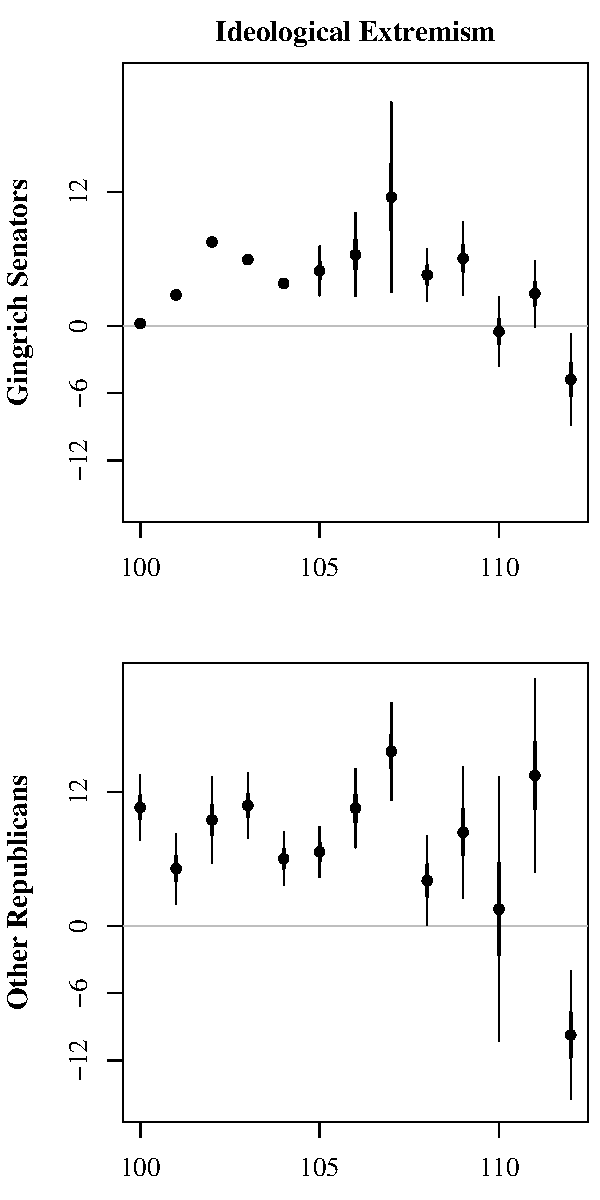
\includegraphics[width = 9cm]{C:/Users/Ethan/Documents/GitHub/partycalls/plots/senate-figure2-gingrich-other-reps.pdf}
\end{figure}

\begin{figure}[H]
	\centering
	\caption{Senate Ideological Extremism Coefficient Plot, Southern and Other Democrats}
	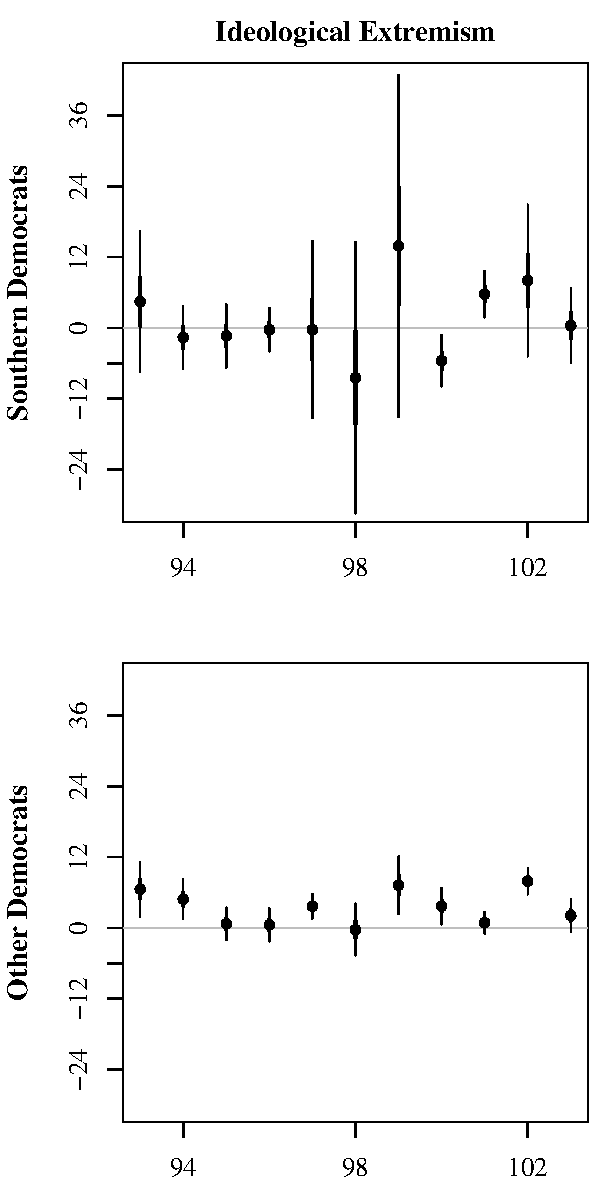
\includegraphics[width = 9cm]{C:/Users/Ethan/Documents/GitHub/partycalls/plots/senate-figure2-southern-other-dems.pdf}
\end{figure}



\end{document}